
\section{Limitless RDD with Historical Data: The Hurricaine \maria\
Death Toll}\label{sec:maria}







Hurricaine Mar\'{i}a struck the island of Puerto Rico on September 20,
2017.
In spite of widespread devistation, for nearly a year after the
hurricaine, the Puerto Rican government officially maintained a
suprisingly low death toll of 64 based on examinations of individual
death reports.
In contrast, several studies by investigative journalists, and academic
researchers, estimated much larger death tolls.
For example, \citet[][; henceforth SLH]{santos2018use} compared monthly death counts recorded in the
months after the hurricaine to historical values, and estimated that
Mar\'{i}a caused 1139 excess
deaths.
In this section, we will reanalyze this dataset to illustrate some
of our ideas, not to suggest an alternative estimate of the death
toll.
(Indeed, this discussion will elide some arguably important
statistical issues that are not directly related to RDD analysis.)

The SLR dataset forms a somewhat unusual regression
discontinuity design, with the months of 2017 as subjects and monthly death
counts $Y_i$, $i=1,\dots,12$, as an outcome.
The running variable $R_i=i$ is month order and months are
``treated,'' $Z_i=1$,
if $R\ge 9$, i.e. if the September 20th hurricaine could possibly have
increased their death counts.
Months prior to September are in the control condition, $Z_i=0$.
Following \citet{neyman:1923} and \citet{rubin1974estimating}, we may
then take each $i$ to have two potential outcomes: $Y_{Ti}$, a potential
response under the treatment condition (the number of deaths that
would occur were $i$ to fall after Mar\'{i}a); and $Y_{Ci}$, a potential response to
control (the death count were $i$ to fall before Mar\'{i}a).
For each $i$, at most one of $Y_{Ci}$ and $Y_{Ti}$ is
observed, depending on $Z_i$; observed responses $Y$ coincide with
$ZY_{T}+(1-Z)Y_{C}$.
% The treatment effect, the number of deaths Mar\'{i}a would cause, in
% the $i$th month is $\tau_i=Y_{Ti}-Y_{Ci}$.

One approach to estimating the death toll from
Mar\'{i}a models $\bm{Y}$ and $\bm{Z}$ as if arising from a randomized
experiment \citep[see, e.g.][for anlogues in the RDD literature]{cattaneo2015randomization,matteiMealliObsStud}.
(Here and throughout, boldface indicates the concatenation of
$n$ realizations of a variable.)
Simple randomization entails ``strong ignorability''
\citep[e.g.][]{rosenbaum1983central}:
\begin{ass}{Strong Ignorability}
\begin{equation}\label{eq:ignore}
Y_{C} \independent Z.
\end{equation}
\end{ass}
For \eqref{eq:ignore} to hold, $R$, which determines $Z$, must be
independent of monthly death counts that would have been observed in
the absense of ``exposure'' to \maria.
That is, \eqref{ignore} implies that month order is irrelevent
to mortality, so that were \maria\ not to strike, any permuation of
monthly death counts would have been equally likely.
Evidence against \eqref{eq:ignore} may be found in the left panel of Figure
\ref{fig:maria}, which plots monthly Puerto Rican death counts from
years 2010--2017.
Seasonal trends are apparent: death counts tend to be higher in the winter
months---particularly Decenber and January---than during the rest of
the year.

Dependence between $R$ and $Y_C$---and hence violations of
\eqref{eq:ignore}---is common in RDDs, and the typical solution to
this problem is to model the mean relationship between $Y_C$ and $R$
(the ``regression'' of ``regression discontinuity'').
This model is fit using the same data, namely $Y$, $R$, and $Z$, that
is used to estimate treatment effects, a practice which leads to a
number of statistical and causal complications.
In this example, we will side-step those complications by exploiting
the historical death counts from years 2010--2016 in the SLR dataset.
The remainder of the paper will discuss the typical case in which such
historical data are not available.

Inspection of Figure \ref{fig:maria} reveals that the relationship
between death counts and month order is non-linear; the structure of
the calendar implies that it is periodical.
Finally, some years appear to be more hazardous overall than others.
To accomodate these factors, we regressed 2010-2016 monthly death counts
on dummy variables for year and a periodic b-spline for month order,
with knots at Februrary, May, August, and November.
Outliers form an additional threat; for instance, death
counts in the final three months of 2014---in particular,
October---were unusually high.\footnote{We do not know why death
  counts were so high in the end of 2014, and are unaware of any
  major event that may have caused those excess deaths. Official data
  on cause of death, reported in \citet[][p. 44]{PRsalud} suggests
  that the difference in total deaths between 2013 and 2014 was almost
  entirely due to deaths caused by common chronic diseases such as
  cancer, heart disease, and diabetes.}
Rather than identifying and removing outliers informally, we fit the regression model
using a robust M-estimation procedure with bounded psi function, which
down-weights and sometimes rejects outliers that would otherwise be
influential \citep{maronna2006robust}%not 100% certain next clause is needed at this point (BH)
, in this way ensuring a bounded influence function \citep{yohaiZamar1997locallyrobustMestimates}.
This model fit is displayed as a dashed black line in Figure
\ref{fig:maria}.

Now let $\hat{Y}_C(R_i)$ be that model's prediction for month $i$ in
2017, and let $\resid_i=Y_i-\hat{Y}_C(R_i)$ be the prediction residual,
with potential values $\resid_C=Y_{Ci}-\hat{Y}_C(R_i)$ and $\resid_T=Y_{Ti}-\hat{Y}_C(R_i)$.
Note that $\hat{Y}_C(R_i)$ cannot itself be influenced by \maria,
since it is based on a model fit to pre-\maria\ death counts \citep[c.f.][]{rebarPaper}.
Hence, the effect of \maria\ on $\resid$ (i.e. $\resid_T-\resid_C$) is exactly equal to its effect on $Y$.
If the model yields unbiased predictions, i.e. $\EE
\hat{Y}_C(R_i)=Y_{Ci}$, then the mean difference
$\bar{\resid}_{Z=1}-\bar{\resid}_{Z=0}$, where $\bar{\resid}_{Z=z}$ is the average
value for $\resid$ of months with $Z=z$, is unbiased for the average number
of deaths per month caused by \maria.
The same is true if the model's predictions in 2017 are biased by a constant,
i.e. $\EE \hat{Y}_C(R_i)=Y_{Ci}+b_0$, for some $b_0\in\mathbb{R}$,
perhaps because of year-to-year trends that were not adaquately
captured by the model.
In short, the hope is that the model fit to monthy death counts from
2010--2016 adequately captures seasonal month-to-month trends in
mortality, leaving $\resid$ as as essentially random.
This may be summarized in a new ignorabilitly assumption:
\begin{ass}{$\resid$-Ignorability}
\begin{equation}\label{eq:ignore2}
\resid_{C} \independent Z.
\end{equation}
\end{ass}
The right panel of Figure \ref{fig:maria} shows residualized death counts $\resid$ as a
function of month order $R$.
Seasonal mean trends are no longer in evidence; \eqref{eq:ignore2} is
thus more plausible than the standard ignorability assumption \eqref{eq:ignore}.

$\resid$-Ignorability decomposes $Y_C$ as the sum of systematic
components---a function of $R$ and disturbances---and relies on the
nature of the decomposition to ensure
that, vis a vis one another, the disturbances and $Z$ may
be regarded as random.
In so doing, residualization mimics the process of ``true'' (as
opposed to pseudo-) random number generation, which derive random
numbers from physical processes that are either chaotic
\citep[e.g.][]{uchida2008fast} or quantum
\citep[e.g.][]{stefanov2000optical}.
When these processes contain an element
of predictability, % \citep{raz2005extractors};
true random numbers are obtained by modeling the predictive component,
and extracting the random component \citep[see, e.g.][]{Nisan1999148}.

\begin{figure}
\centering
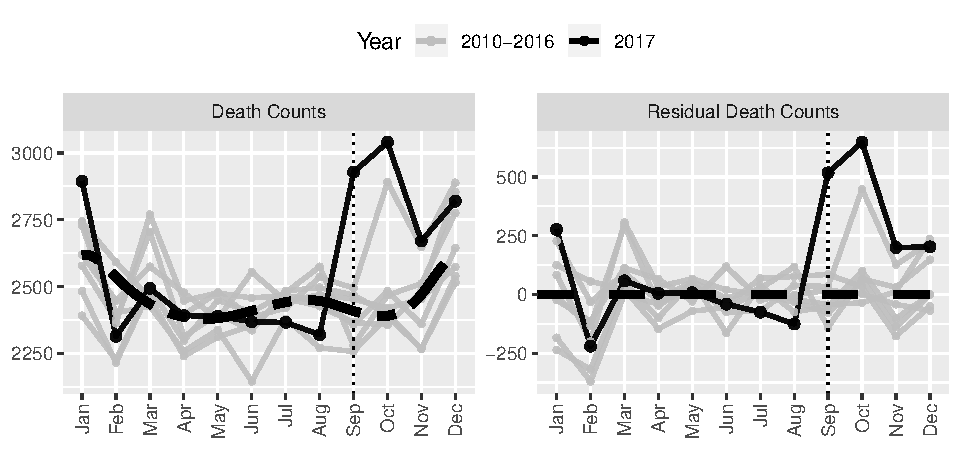
\includegraphics[width=0.95\textwidth]{maria.pdf}
\caption{Monthly death counts in Puerto Rico from years 2010--2017, before and after
  residualization. The plot on the left shows monthly death counts,
  adjusted for month length. A vertical dotted line denotes September,
  the month \maria\ hit. The fit of the robust model described in the
  text is shown as a dashed black line. The plot on the right shows
  the monthly residuals of the model fit, with a dashed line denoting
  zero.}
\label{fig:maria}
\end{figure}


\subsection{Estimating Effects Under Ignorability}\label{sec:rand}

\marginpar{I commented out the material about Fisher, which is kinda
  ancillary (no pun intended)}



To continue in the manner of Neyman
\citeyearpar{neyman:1935}, one conditions on the realized sizes
$N_{1}$ and $N_{0}$ of the treatment and control group samples, where
 $N_{j} \equiv \sum_{i=1}^{n} \indicator{Z_{i}=j}$, and on vectors of
 potential outcomes $\bm{\resid_C}$ and $\bm{\resid_T}$, thereby modeling
 potential outcomes as non-stochastic.
In fact, a weaker conditioning set suffices; let
$\mathbf{A}^{*}=\{N_{1},N_{0},\tilde{\mathbf{\resid}}_{T},\tilde{\mathbf{\resid}}_{C}\}$,
where  $\tilde{\mathbf{\resid}}_{T} = \mathbf{\resid}_{T} - \bar{\resid}_{T}$ and
$\tilde{\mathbf{\resid}}_C$ are centered potential outcomes.
This centering is around study population means,
$\bar{\resid}_{T} = n^{-1}\sum_{i}\resid_{Ti}$ and
$\bar{\resid}_{C} = n^{-1}\sum_{i}\resid_{Ci}$, as opposed to within-group means
$\overline{(\resid_{T})}_{Z=1}$
and
$\overline{(\resid_{C})}_{Z=0}$.
As a result, $\tilde{\mathbf{\resid}}_{T}$ and $\tilde{\mathbf{\resid}}_{C}$ are
entirely unobserved, in contrast with $\bm{\resid_C}$ and $\bm{\resid_T}$, which
are at least partially observed.
However, under null hypotheses of the form $H_\tau$ that specify
average treatment effects $\tau=\EE Y_T-\EE Y_C$, conditioning
on $\mathbf{A}^{*}$ allows for randomization- (if not permutation-)
based inference.

Consider the archetypical
Neyman-type test statistic \citeyearpar{neyman:1923,neyman1934stratifiedsampling}, %is
  % If $\tilde{\mathbf{y}}_H$ denotes the potential response
  % $\mathbf{y}_{c}$ that would be entailed by a strong null $H$, in
  % combination with observations $\mathbf{y}$ and $\mathbf{d}$, then
\begin{align} \label{eq:tudef}
t_{u}({\mathbf{y}},\mathbf{z}) &=
\frac{\bar{\resid}_{z=1} -
                             \bar{\resid}_{z=0}}{
\mathrm{SE}_{u} \left\{ \bar{\resid}_{Z=1} -  \bar{\resid}_{Z=0} \right\}
                             },\, \text{where}
\\
%% where $\overline{v}_{z=j} = n_{j}^{-1} \sum_{i: z_{i} = j}
%% v_{i}$, $n_{j} = \sum_{i}\indicator{z_{i} =j}$, for $j = 0, 1$, and
\mathrm{SE}_{u}^2 \left( \bar{\resid}_{Z=1} -  \bar{\resid}_{Z=0} \right) &= \frac{s_{z=1}^{2}({\mathbf{\resid}})}{n_{1}} +
    \frac{s_{z=0}^{2}({\mathbf{\resid}})}{n_{0}}  \label{eq:sudef}
% \\
%     s_{z=j}^{2}(\mathbf{v}) &= \frac{1}{n_{j}-1}\sum_{i: z_{i} = j}
% (v_{i} - \bar{v}_{z=j})^{2} .\nonumber
% \end{equation}
\end{align}
is the ordinary unpooled two-sample variance. With conditioning on
$\mathbf{A}^{*}$, and assuming \eqref{eq:ignore2}, the expected value
of \eqref{eq:sudef} is
${s^{2}({\mathbf{\resid}_{T}})}/{N_{1}} +
{s^{2}({\mathbf{\resid}_{C}})}/{N_{0}}$, an upper bound of the variance of
$\overline{(\resid_{T})}_{Z=1} - \overline{(\resid_{C})}_{Z=0}$, conditional on
$\mathbf{A}^*$.

Under this approach, we can construct assymptotic tests of null
hypotheses that specify average treatment effects.
For instance, under $H_{0}:\EE Y_C=\EE Y_T$ (or
equvalently $\EE \resid_C=\EE \resid_T$), and assuming \eqref{eq:ignore2},
$t_{u}(\mathbf{\resid}, \mathbf{Z})\stackrel{d}{\rightarrow}\mathrm{Normal}(0,v)$,
some $v\leq 1$, conditional on $\mathbf{A}^{*}$; see
Appendix~\ref{apnd:RICLT}.
More generally, for any $\tau$ we can assess
$t_{u}(\mathbf{\resid}-\tau\mathbf{Z}, \mathbf{Z})$ against a standard Normal
or central $t$ distribution to test
$\bar{H}_{\tau}: \EE Y_T-\EE Y_C=\tau$.

Such tests can serve as foundation for both point and interval
estimates of average treatment effects.
The value $\hat{\tau}_{\text{HL}}$ for which $t_{u}(\mathbf{\resid}-\hat{\tau}_{\text{HL}}\mathbf{Z},
\mathbf{Z})$ is equal to its null expected value of 0 is a Hodges-Lehmann estimate of the true average effect\footnote{The general definition of
Hodges-Lehmann estimates is more elaborate, also addressing eventualities
of there being no such $c$, or of its failing to be unique
\citep[e.g.,][Sec.~2.7.2]{rosenbaum:2002}}.
In this case, this $\hat{\tau}_{\text{HL}}$ is simply the difference in means between the
control and treatment groups, $\bar{E}_{Z=1}-\bar{E}_{Z=0}$.
The set \{$\tau$: $H_{\tau}$ is not rejected at level $\alpha$\}, typically an interval, is a
$100(1-\alpha)\%$ confidence set for the average treatment effect.

Though this inferential approach is assymptotic, arguments in
Appendix~\ref{apnd:RICLT} suggest that it is conservative in small
samples;  in any event, we may use it to estimate the \maria\ death
toll, if only as an illustration.
In the first eight months of 2017, the average residual death count
was roughly
$\bar{\resid}_{Z=0}=$-9 deaths;
in the final four months, we have
$\bar{\resid}_{Z=1}=$396
deaths, implying an estimated death toll of 405 deaths
per month, or a total of 1620 deaths.
Comparing
$t_{u}(\mathbf{\resid},\mathbf{Z})=$3.5
to a t-distribution with 3.9 degrees
of freedom gives a two-sided p-value of 0.027
testing the null hypothesis of no excess deaths
average.
Inverting the t-test gives a 95\% confidence interval of
[77, 732] excess deaths per
month, or a total death toll of
[308, 2930].

In the \maria\ dataset, there was no distinction between treatment
assignment and compliance.
However, in many experiments and in so-called ``fuzzy'' regression
discontinuity designs, subjects assigned to treatment do not always
receive it.
In that case, let $D_{i}$ denote the treatment $i$ actually
received --- the ``dose.''
This $D$ is an intermediate outcome, so there are
corresponding potential outcomes $D_{C}$ and $D_{T}$, with $D \equiv ZD_{T}
+ (1-Z)D_{C}$.
Subject $i$ is a non-complier if $D_{Ci}=1$ or $D_{Ti}=0$, though we
will assume the monotonicity condition $D_{C}\equiv 0$ --- there may be
subjects assigned to the treatment who avoid it, but no one gets
treatment without being assigned to it.
We shall also posit the exclusion restriction,
that $Z$ influences $Y$ only by way of its effect on $D$
\citep{bloom1984ans,Angrist:etal:1996,imbens:rose:2005}.
Our focus of estimation is the
 ``treatment-on-treated'' effect (TOTE), $\EE(Y_{T} - Y_{C}|
 D_{T}=1)$.
Then, we test hypotheses of the form
$H_{\tau}: \EE( Y_{T} - \tau D_{T}) =\EE (Y_{C} - \tau D_{C})$ by
comparing $t_{u}(\mathbf{\resid}-\tau\mathbf{D}, \mathbf{Z})$ to the
appropriate sampling distribution.
Although in the case of full compliance $\bm{D}\equiv\bm{Z}$ the
Hodges-Lehmann estimator
$\hat{\tau}_{\text{HL}}$ is equal to the difference in means of
$\resid$ between the treatment and control groups, the same cannot
always be said when $\bm{D}\ne \bm{Z}$.
Similarly, the
confidence interval or set induced by~\eqref{eq:tudef} requires a distinct explicit
test for each of a range of $\tau$s
\citep[Sec.~7]{imbens:rose:2005,baiocchiChengSmall2014IVtutorial}.


\section{Limitless RDD: The Typical Case} \marginpar{This section
  needs to be renamed}

Our estimate of the Hurricaine \maria death toll in Puerto Rico relied
heavily on the availability of seven years of historical monthly death
counts preceeding 2017.
That analysis effectively partioned the data into two parts: pre-2017
data was used to fit a model for $Y_C$ as a function of
$R$, and 2017 data was used to estimate effects.
Partioning the data such allowed us to partition the methods:
specifically, the causal inference in Section~\ref{sec:rand} made no
reference to the fitting procedure in the historical data, and instead
treated its outputs as a given.
This data structure atypical---for instance, the LSO dataset does not include a
historical component in which no treatment was present.
Instead, typical RDD analysis uses the same data to both estimate the
regression of $Y_C$ on $R$ and to estimate treatment effects.
Then, it is inadvisable to estimate effects without accounting for the
depencencies induced over the course of model fitting.

This section will extend the approach of the \maria\ analysis to the
more common situation in which both regression model fitting and
effect estimation use the same dataset.
Doing so will involve subtle but important modifications of the
$\resid$-ignoriability assumption and the analysis steps that build on
it.
This analytic strategy requires careful attention to the details of
the model-fitting process; we will argue for the general applicability
of robust regression with a bounded influence function.


\subsection{An Analytic Model for RDDs} \label{sec:model-eey-c-r}

Suppose the statistician to have selected a \textit{residualizing procedure}: a
trend fitter, i.e. a function of
$\{({y}_{i},d_{i},r_{i})\}_{i=1}^{n}$ returning
fitted parameters $\hat{\theta}$ in a sufficiently regular
fashion, along with a
family $\{\dt{\cdot}{\cdot}: \theta\}$ of residual or partial
residual transformations, each mapping data $(\mathbf{y}, \mathbf{r})$ to
$\{\dt {y_{i}}{\mathbf{r}} \}_{i=1}^{n}$.
Appendix~\ref{sec:large-sample-rand}
%\citet[\S~\ref{sec:large-sample-rand}]{lrdauthors:supp}
states the
needed regularity condition, which is ordinarily met by OLS and always
met with our preferred fitters (Section~\ref{sec:test-hypoth-no}).
Causal inferences taking
the perspective that $Z$ is random due to
randomness in $R$ are then possible under the following assumption.

\begin{ass}{Residual Ignorability}
\sloppy
Given a residualizing procedure $(\hat{\theta}, \dt{y}{r})$,
\begin{equation}\label{ycheck}
\dt[\thetaInf]{Y_{C}}{ R }%\mathbf{\Ych}_{C}
\independent {Z},
\end{equation}
where $\thetaInf$ is the probability limit of $\hat\theta$.
\end{ass}
Residual Ignorability states that, though $Y_C$ may not be independent of
$Z$,  it admits a residual transformation bringing about such
independence.   With $\dt[\hat\theta]{Y_{C}}{ R}$ a suitable
partial residual, Residual Ignorability is entailed by the
\textsc{ancova} model (\S~\ref{sec:robust-analys-covar}), or by the combination of any parametric model
for $\EE (Y_{C}| R)$ with a strict null $H$ relative to which the
value of $Y_{C}$ can be reconstructed from the values of $Y$, $D$ and
$Z$ (\S~\ref{sec:randProc}).
(In either of these cases $\dt[\thetaInf]{Y_{C}}{ R}$
is independent not only of $Z$ but also $R$,
a modest strengthening of~\eqref{ycheck}.)


\sloppy
Assuming Residual Ignorability, inference about treatment effects is
made conditionally, on
$\mathbf{A}= (\dt[\thetaInf]{\mathbf{Y}_{C}}{ \mathbf{R}}$, $\mathbf{D}_{T})$.
Conditioning on
$\dt[\thetaInf]{\mathbf{Y}_{C}}{ \mathbf{R}}$
removes little of the entropy
in $\mathbf{R}$, leaving it available as a basis for inference.
Uncoupled to $Y_{T}$s, the detrended  $Y_{C}$s,
$\dt[\thetaInf]{\mathbf{Y}_{C}}{ \mathbf{R}}$,
are in themselves uninformative about $\EE(Y_{T} - Y_{C})$, so
the variables comprising $\mathbf{A}$ are jointly
%\marginpar{$\leftarrow \Delta$ to $(\mathbf{Y}_{C}, N_{0}, N_{1})$?}
S-ancillary, just as $\mathbf{A}^{*}$ was seen to be
in Section~\ref{sec:randProc}.  As in Neyman-style randomization inference for RCTs, some conditioning variables are
unobserved; but this is not an impediment, at least for large-sample
inferences.



\subsection{Inference About the Treatment Effect}
\label{sec:test-hypoth-no}

For inference about $\tau$ under the model
$Y_{T} = Y_{C} + \tau D_{T}$, select a specification
$\mu_{\beta}(\cdot)$ for $\EE(Y_{C}| R)$,
such as the
linear model $\mu_{\beta}(R) =\beta_{0} + R\beta_{1}$.


Separately for each hypothesis $H: \tau=\tau_0$ under
consideration, one calculates
$\mathbf{y}_{H} = \mathbf{y} - \mathbf{d}\tau_{0}$, then
applies the chosen specification and fitter to
$(\mathbf{y}_{H}, \mathbf{r})$.
The combination of the data, the
model fit, and the residual transformation $\dt{\cdot}{\cdot}$ give rise to residuals
$\dt[\hat\theta]{\mathbf{y}_{H}}{\mathbf{r}}$, completing the
residualizing procedure. Whether $H$ is rejected or sustained is
determined by the value of the sandwich-based \textsc{ancova} $t$-statistic
\eqref{eq:tedef}.

In practice it is expedient to use a near-equivalent
test by modifying the residualizing
procedure.
When regressing $Y_{H}$ on $R$, include an additive
contribution from $Z$, so that $\mu_{\beta}(R) =\beta_{0} +
R\beta_{1}$ is replaced with $\mu_{(\beta,\gamma)}(R) =\beta_{0} +
\beta_{1}R + \gamma Z$. With sandwich estimates of
$\text{Cov}\{(\hat{\beta}_{H}, \hat{\gamma}_{H})\}$,
the t-ratio comparing $\hat{\gamma}_{H}$ to
$\text{SE}_{s}(\hat{\gamma}_{H})$ induces a generalized score test \citep{boos1992genscoretest}. Implicitly it is a two-sample
t-statistic with covariance adjustment for $R$, as in \eqref{eq:tedef}: with fitting via OLS,
this correspondence would be exact, as noted in Section~\ref{sec:robust-analys-covar}; with the robust MM estimation we
favor, the correspondence is one of large-sample equivalence
(Appendix~\ref{sec:suppl-s-refs}).
Iterative testing is facilitated by regressing $\mathbf{y}$ on $\mathbf{r}$ and $\mathbf{z}$
with offset variable $\mathbf{d}\tau_{0}$; then only the offset needs to
be modified to test $H: Y_{T} = Y_{C} +  \tau D_{T}$ for a new $\tau$.

\subsection{Post-Fitting Diagnostics} \label{sec:post-fitt-diagn}
Once the Hodges-Lehmann estimate $\hat{\tau}_{\mathrm{HL}}$ has been found, one
inspects the corresponding regression fit for points of high influence.
Bounded influence regression is helpful here.  Besides making
influential points easier to see in residual plots, this limits
effects of data contamination, as non-conforming influence points are
down-weighted as a result of the fitting process. This down-weighting
is reflected in robustness weights, ranging from 1, for non-discounted
observations, down to 0, for the most anomalous observations.
Plotting % As
% an indicator of robustness to non-constant effects.
% (But is this overloading the discussion here?)
robustness weights against residuals may expose opportunities to
improve the fit of $\mu_{\beta}(R)$, or of the treatment effect model;
plotting them against $R$ may expose contaminated sub-regions
of $\mathcal{W}$ that specification testing failed to remove.


\subsection{Robust Estimation of $\EE (Y_{C}| R)$}
\label{sec:robust-altern-ordin}
If moderate sample contamination may be present --- specifically, contamination of
a $O(n^{-1/2})$-sized
share of the sample --- consistent estimation of $\thetaInf$ requires a
bounded influence fitter (\citealp[Thm.~3]{he1991localbreakdown};
\citealp{yohaiZamar1997locallyrobustMestimates}), as opposed to
maximum likelihood.  OLS does not meet this consistency requirement;
nor do many robust regression methods engineered to meet
objectives other than bounding the influence function
\citep{stefanski1991note}.
Further, no specification test is powerful enough
to reliably detect contamination of this size; power to detect anomalies
affecting only $O(n^{-1/2})$ of the sample can only tend to a number
strictly less than 1.  %NB: This is expanded a little in a
                       %now-commented-out passage of Discussion, the
                       %on referencing vdvaart:1998.
Thus under uncertainty about the
proper limits of $\mathcal{W}$, MM-estimation (\S~\ref{sec:robust-altern-ordin}) is to be preferred.
The analyses and simulations presented below use MM-estimators with bisquare $\psi$ and
the ``fast S'' initialization of \citet{salibian-barreraYohai2006fastS}.

\sloppy
Assumptions about the form of $\EE[(Y_{T}, Y_{C}) | R]$ are not
readily dispensed with;
% Statistic (\ref{eq:tedef}) is often computed using a portion of the
% available data, a subset $\mathcal{W} \ni c$ of the support of $R$
% \citep[e.g.][]{imbens2008regression}.
even nonparametric RDD models
%take $R$ to follow a continuous distribution, and
place continuity and smoothness restrictions on $\EE(Y_{C}| R=r)$ \citep[\S~5]{lee2008regression, kolesarRothe17}.
On the other hand, methods discussed in Sec~\ref{sec:robust-analys-covar} continue to
apply if $\EE (Y_{C}| R) = \alpha + R\beta$ is relaxed to
$\EE (Y_{C}| R) = \alpha + \vec{f}(R)\beta$, for
$\vec{f}(\cdot)$ a $1 \times k$ vector valued function.
Unfortunately, if the model is fit by OLS, then such relaxation of assumptions can have the unwelcome
side-effect of undercutting the robustness of the analysis.  The
reasons have to do with mechanics of regression fitting.

Polynomial specifications
$\EE(Y | R=r) = \sum_{j=0}^{J} r^{j} \beta_{j}$ are common but often
problematic; in combination with ordinary least squares fitting, they
implicitly assign case weights that can vary widely and
counterintuitively \citep{gelman2016high}.
This liability is already
in evidence with $J=1$, the linear specification, where leverage
increases with the square of $r -\bar{r}$.  With an analysis sample
of the form $\{i : R_{i} \in \mathcal{W}\}$ for a ``window''
$\mathcal{W} \ni c$, if $\mathcal{W}$ is slightly too wide then the
sample is contaminated near its outer boundaries, precisely
where leverage is at its highest.

In order to identify leverage points that are also influential,
OLS fitting is sometimes combined with specialized diagnostics such as
plots of Cook's distances
 \citeyearpar{cook1982residuals}. An alternate remedy, playing
 an important role in this paper, is to fit the
 specification using a modern MM,  SM, or similar estimator so designed
 as to possess a bounded influence function
 \citep{yohaiZamar1997locallyrobustMestimates}; such procedures address influence
 in the course of the fitting process.
 % Diagnostics such as inspection of Cook's distances
 % \citeyearpar{cook1982residuals} can identify leverage points that are
 % also influential.  In regression problem other than RDDs, a natural
 % remedy is to select $\vec{f}(\cdot)$ as a spline basis, thus fitting
 % a piecewise rather than a global polynomial
 % \citep{ruppert2003semiparametric}.  For the purpose of estimating
 % $Z$'s contribution to $\EE (Y|R,Z)$, this is similar in its effects
 % to retaining the global polynomial specification while narrowing $\mathcal{W}$
 % until it does not straddle knots of the chosen spline basis.
In MM-estimation as in OLS,
coefficients $\beta$ of a linear specification solve estimating equations
$\sum_{i} \psi\left\{ ({y}_{i} -
\vec{x}_{i}\beta)/s \right\} \vec{x}_{i} =0$, where $s>0$ and
$\psi(\cdot)$ is an odd function satisfying $\psi(0)=0$,
$\psi'(0)=1$ and $t\psi(t)\geq 0$; bounded influence fitters replace OLS's $s\equiv 1$ with resistant preliminary
estimates of residual scale, and OLS's $\psi(t) = t$ with a continuous $\psi$
that satisfies $\int_{0}^{\infty}\psi(t)dt < \infty$. This limits
the loss incurred by the fitter for failing to adapt itself to a small
portion of aberrant observations;
% e.g. Huber's $t \mapsto \mathrm{sign}(t) * \min(|t|, 1.345)$
% \citeyearpar{huber1964robust}.  Capping the influence of any one observation
% requires that $\psi$ be not only bounded but
% \textit{redescending}. A redescending $\psi(t)$
% increases smoothly from 0 as $t$ increases from 0, but for
% sufficiently large $t$ it levels out and redescends, reaching 0 at
% some $t_{r} < \infty$; $\psi(t) = 0$ for all $t>t_{r}$.
it is permitted to instead systematically down-weight them. When
present, such aberrancies present large residuals, that are easier to
see in ordinary diagnostic plots, and small
``robustness weights,'' an additional diagnostic not available for OLS fitting
\citep{maronna2006robust}.  We are not aware of prior work addressing
potential contamination of an RDD sample with the assistance of
bounded influence MM-estimation.

Surprisingly, given their common origins in %the work of
Huber \citeyearpar{huber1964robust}, MM estimation is not routinely
paired with sandwich estimates of variance, as in \eqref{eq:tedef} and
the surrounding discussion of \S~\ref{sec:robust-analys-covar}.
Exceptions include Stata's \texttt{mmregress} and R's \texttt{lmrob},
which optionally provide Huber-White standard errors
\citep{verardiCroux2009robust,rousseuwetal2015robustbase}.

\section{Assessing the Plausibility of Residual Ignorability}

\subsection{Specification Tests}\label{sec:specification}

Analysis of RCTs and quasiexperiments often hinges on assumptions of
independence of
 $\mathbf{Z}$ from $(\mathbf{X}, \mathbf{Y}_{C}, \mathbf{Y}_{T})$.
%% Analogous statements will hold for more complex randomization or
%% ignorability assumptions as well.
 Although neither $\mathbf{Z} \independent \mathbf{Y}_{C}$ nor
 $\mathbf{Z} \independent \mathbf{Y}_{T}$ can be directly tested,
 since potential outcomes are only partly observed, assumptions of form
 $\mathbf{Z} \independent \mathbf{X}$ are falsifiable: researchers can
 conduct placebo tests for effects of $Z$ on $X$.
% Just as $H: \mathbf{y}_{T} - \mathbf{y}_{C} =
% \mathbf{\tau}$ is tested in the strong randomization inference
% paradigm, the researcher might assess imbalance in a covariate, as measured
% either by the difference of means,
% $\bar{x}_{Z=1} - \bar{x}_{Z=0}$, or by the difference of means in a transform of
% the covariate, $\overline{\dt[\thetaInf]{\mathbf{x}}{\mathbf{r}}}_{Z=1} - \overline{\dt[\thetaInf]{\mathbf{x}}{\mathbf{r}}}_{Z=0}$,
% to the distribution of the same difference under permutations of
% $\mathbf{z} $.
Of course, treatment cannot affect pre-treatment variables; this is
model-checking (%\citealp{bayarriBerger2000pvalues};
\citealp[][\S~5.13]{cox2006pos}%; \citealp[][Ch.~6]{gelman:etal:2004};
%\citealp[][Ch.~14]{lehmannRomano2006TSH}
).  Here as
 elsewhere \citep{box1980sab}, checks finding fault with a model prompt
 refinement, not abandonment; refinements typical of RDD analysis remove portions of
 the sample that are suspected of contamination.

%% BELOW APPEARED IN R2
% With $k>1$ covariates $\mathbf{x}_{1}, \ldots, \mathbf{x}_{k}$, issues
% of multiplicity come into play: if a test of the hypothesis that $(X_{1}, \ldots, X_{k})$
% are independent of $Z$ rejects whenever any of the $k$
% level $\alpha$ tests is rejected, then its type 1 error rate may
% greatly exceed $\alpha$.  Because the tests are non-independent, with
% covariances that (except in the differences-of-means case) may be
% difficult to estimate, we combine them with a simple Bonferroni
% correction.
%% BELOW HAD BEEN WRITTEN FOR R2 AND THEN EDITED OUT
%% One solution is to combine the $p$
%% test statistics $\overline{(\mathbf{x}_{1})}_{z=1} - \overline{(\mathbf{x}_{1})}_{z=0}$, \ldots, $\overline{(\mathbf{x}_{p})}_{z=1} - \overline{(\mathbf{x}_{p})}_{z=0}$
%% into one statistic $t(\mathbf{x}, \mathbf{z})$, then conduct a
%% single test based on it.
%% %For comparing
%% %3 or more treatment conditions while controlling the family-wise error rate, a
%% %common device is to use the ``max-t'' statistic, i.e. test based on $t(\mathbf{x},
%% %\mathbf{z}) = \max_{k} (t(\mathbf{x}_{\cdot,k}) -
%% %\EE_{0}T(\mathbf{x}_{\cdot,k}))/\var^{1/2}_{0}(T(\mathbf{x}_{\cdot,k}))
%% %$ \citep{hothorn2008simultaneous};
%% %In a discussion of covariate balance specifically,
%% \citet{hansen:bowers:2008} recommend a combined statistic
%% along the lines of Hotelling's
%% \citeyearpar{hotelling1931generalization} $T^2$, $d^{2}(\mathbf{x}, \mathbf{Z})$, that follows a large-sample chi-squared
%% distribution under the hypothesis that $\mathbf{X} $ is
%% independent of, and unaffected by, $\mathbf{Z}$.
%% %% Other solutions
%% \citep[\textit{e.g.,}][]{rosenbaum2005exact} involve testing with a
%% statistic $t(\mathbf{x}, \mathbf{z})$ that is not directly related to
%% the univariate statistics.

 Writing in the RDD context, \citet{cattaneo2014randomization} test
 for marginal associations of $\mathbf{Z}$ with covariates $\mathbf{X}_{i}$,
 $i=1, \ldots, k$, using the permutational methods that are applied
 in Fisherian analysis of RCTs.
% Specifically, they
%  obtain p-values though \eqref{eq:01}, with test statistics
%  $t(\mathbf{x}_{i}, \mathbf{z}) = |\overline{(x_{i})}_{z=1} -
%  \overline{(x_{i})}_{z=0}|$,
%  $ i \leq k$, after conditioning on $\mathbf{X}$ in addition to
%  $\sum_{i} Z_{i}$.
Relatedly, \citet{lee2010regression} recommend a
 tests for conditional association, given $R$, of $\mathbf{Z}$ and
 $\mathbf{X}$, by fitting models like those discussed in
 \S~\ref{sec:robust-analys-covar} for impact estimation, but with
 covariates rather than outcomes as independent variables%
%, they incorporate covariance adjustments for $R$
. %, testing
 %whether these regressions' $z$ coefficients are plausibly
 %0.
Viewing the $R$-slopes and intercepts as simultaneously estimated
 nuisance parameters, these are balance tests applied to
 the covariates' residuals, %net of linear association with $R$,
rather than to the covariates themselves.

%Whether covariates or covariate residuals are assessed for lack of
%correlation with $Z$,
If there are multiple
covariates there will be several such tests. To summarize their
findings with a single p-value, the
regressions themselves may be fused within a
``seemingly unrelated regressions'' model, followed by a test of the
intersection hypothesis that each regression's $z$-coefficient is 0
\citep{lee2010regression}, or the
separate tests' p-values could simply be combined using the Bonferroni
principle.  Li et al.'s
\citeyearpar{liMatteiMealli2015BayesianRD} RDD method wraps
its specification checking steps into a Bayesian model. % that is also used for effect
%estimation.
This approach addresses multiplicity of placebo tests as a matter of course; as with the method of \citet{cattaneo2014randomization}, however, its implied placebo tests, of whether $Z$ ``affects'' $\mathbf{X}$, are not covariance adjusted for $R$.


McCrary's test for manipulation of treatment assignments
\citeyearpar{mccrary2008manipulation} can be understood as a %lack of
%association test applied over an $\{|R| < b\}$ window.
placebo test with the density of $R$ as the independent variable.
The test's
purpose is to expose the circumstance of subjects finely manipulating their
$R$ values in order to secure or avoid assignment to treatment.  Absent
such a circumstance, if $R$ has a density then it should appear to be
roughly the same just below and above the cutpoint.  McCrary's
\citeyearpar{mccrary2008manipulation} test statistic is the difference
in logs of two estimates of $R$'s density at 0, based on observations
with $R<0$ and $R>0$ respectively.
% Inspection of the form of these
% estimates reveals that, but for the presence of the logarithms, the
% statistic also is a difference of means over observations with
% $Z_{i}=0$ or $1$, in both cases with $|R|$ as the quantity being
% averaged.  (The two means are calculated with weighting, with weights
% %set to 0 for $|R|>b$ and otherwise
% determined by the combination of a
% chosen kernel and bandwidth and simultaneously estimated nuisance parameters; see
% McCrary's [\citeyear{mccrary2008manipulation}] equation 4.)
Manipulation is expected to generate a clump just beside the cut
point, on one side of it but not the other, and this in turn engenders
imbalance in terms of distance from the cut-point.


In practice, specification test failures inform sample exclusions.
%: failed density tests lead to exclusions around the cut
%point; failed placebo tests lead to narrower widths of analytic
%windows.
Failures of the density test are addressed by restricting
estimation to observations with $|R|>a$, some $a \geq 0$
\citep[e.g.,][]{barrecaetal2011birthweightRDD,eggers2014validity}.
When balance tests fail,
\citet{lee2010regression} would select a window
$\mathcal{W} \subseteq [-b, b]$, $b>0$, % using
% a method that anticipates possible non-linearity in $\EE (X | R=r)$
% outside a neighborhood of 0,
and repeat the test on $\{i : r_{i} \in \mathcal{W}\}$. Similarly,
\citet{cattaneo2014randomization} recommend testing hypotheses
$H_{b_{i}}: {X} \independent {Z}| \{|R| < b_{i}\}$, $b_1 > b_2 > \cdots >0$, in sequence,
proceeding until identifying  $b = \max \{ b_i: H_{b_{i}}$ is not rejected$\}$;
the analytic sample is then restricted to  $\{i: r_{i} \in (-b,b)\}$.
%This method's tests of each $H_{b_{i}}$ are neither covariance
%adjusted nor multiplicity corrected.
The analyst decides whether this test-and-reduce process
should begin in the middle of $\mathcal{W}$ or at its boundaries.

% The $\alpha$ level used for these tests may differ from the
% $.05$ that is conventional in outcome analysis;  \citet{cattaneo2014randomization} use $\alpha=.15$.
% Whatever the choice of $\alpha$, Berger's sequential intersection
% union principle \citep{rosenbaum2008testing,hansenSales2015cochran} entails that the sizes of $H_{b*}$, and of each
% of the $H_{b}$ rejected prior to testing $H_{b^{*}}$, are not inflated
% by the multiplicity of tests within the family $\{H_{b}: b\}$.

% McCrary's specification test focuses on the center of the RDD window,
% rather than its boundaries \citep{mccrary2008manipulation}.
% It is designed to test whether subjects consciously sort around the
% cutoff by manipulating their $R$ values explicitly.
% It does so by examining whether an unexpectedly large or small number
% of subjects find themselves just barely on one side of the cutoff or
% the other.
% When the running variable is discrete, for each value $r$ in the support of $R$,
% let $n_R(r)$ denote the number of subjects $i$
% with $R_i=r$, i.e.,  $|\{i:r_i=r\}|$; continuous $R$s are binned prior to the
% test.  Next, $n_{R}$ is used as the outcome of a preliminary RDD
% analysis, modeled using local linear regression as a function
% of $r$ on either side of $c$. The test asks whether there is a discontinuity at $c$:
% a change in $n_{R}$ larger than chance could produce suggests subjects
% may have manipulated $R$ to control their treatment assignments,
% perhaps invalidating the analogy to a controlled experiment.
%% [clipping the below to save a little space; I think it works w/o it.]
%% A McCrary test failure is neither necessary nor sufficient to show
%% that subjects sorted around the cutoff; however, it is suspicious.




\subsection{Checking and Refining the Window ($\mathcal{W}$)}
\label{sec:bandwidthChoice}

If subject matter knowledge suggests that chance variability intrinsic
to $R$ is typically of magnitude $b$, then RDD modeling focused on
distilling local randomization might set $\mathcal{W}$ to $[-b,b]$. But it
is also sensible to subject such an initial choice to specification
testing (\S~\ref{sec:specification}).%\marginpar{I replaced $c$ here
%  with $b$ since $c$ is the cutoff-AS\\ ---Good catch thnx! -B}

Common RDD specification checks
can be regarded as testing Residual Ignorability with a multivariate
``outcome'' $Y^{*}$ combining the actual outcome $Y$ with covariates $X$---\eqref{ycheck} with
$\mathbf{Y}_{C}^{*} = (\mathbf{X}, {Y}_C)$ in place of $Y_{C}$.
% perhaps with minor adjustment to the forms of $\dt[\theta]{ \cdot }{ r}$
% and corresponding fitter $\hat{\theta}(\cdot, R)$.
%
%In addition to $\mathcal{W}$, researchers must pick $f$, a model for $Y_C$.
%% If a lagged outcome is not available, the data will not have informed the specification of
%% $\EE (Y_{C}| R=r) $ on the treatment side of the threshold.  It
%% should be treated as an approximation, and $\mathcal{W}$
%% deliberately chosen to be narrow enough to limit influences of errors
%% of approximation, as distinct from errors of estimation, on statistics
%% $t({\mathbf{y}_H} - f(\mathbf{r}; \theta(\mathrm{r},
%% {\mathbf{y}_H}))$.
%% Covariate placebo tests can be helpful in this regard.
This calls for preliminary residualizing procedures, mechanisms to
decompose  $X$ into components that are systematic or unpredictable,
vis a vis $\mathbf{R}$, just as ${\mathbf{Y}_C}$ will later be decomposed.
%% Since $Z$ cannot have an effect on a pre-treatment
%% covariate, the preliminary step of reconstructing
%% $x_{C}$ is not needed.
%%% [Reorg obviated need for the above, as this passage now precedes
%%% discussion of reconstructing Y_C]
Our analysis of the LSO data posits systematic components that are
linear and logistic-linear in $R$, depending on whether $X$ is
a measurement or binary variable. %, paralleling its choice of a linear decomposition
% for the primary outcome, subsequent GPA.  (It is fitting that the $X$- and
% $Y$-specifications mirror each other in model complexity.)
The placebo check adds $Z$ to the specification and tests whether its
coefficient is zero.  We implement these checks as Wald tests with
heteroskedasticity-robust standard errors, as in
\S~\ref{sec:robust-analys-covar}, using the Bonferroni method to
combine placebo checks across covariates.
% yielding a test of the
% hypothesis that all of the covariates' residuals are jointly ignorable within the
% given $\mathcal{W}$.

If the first window tested has form $\mathcal{W} = (-b, b)$,
write $H_{b}$ for the corresponding joint ignorability hypothesis.
If the $R$-adjusted covariate placebo tests reject $H_{b}$ then the process is repeated for
$\mathcal{W}' = (-b', b')$, some
$b' < b$, and perhaps repeated again if $H_{b'}$ also is rejected.
This may seem to call for a further layer of multiplicity correction,
since any number of
bandwidths may have been tested before identifying a
$b$ for which $H_{b}$ is sustained; but it so happens that this form
of sequential testing implicitly corrects for multiplicity, according to the
sequential intersection union principle
(\citealp[SIUP;][Proposition~1]{rosenbaum2008testing};
\citealp{hansenSales2015cochran}). To compensate for conservatism of
the Bonferroni method, we test with size
$\alpha_{B}=.15$, not $.05$.
% Let
% $\{b_{1}, b_{2}, \ldots\} \subseteq (0, \infty)$ be a descending sequence of
% candidate bandwidths, with an accompanying family $\mathcal{B}$ of
% tests, one for each $H_{b}$. Define a modified family $\mathcal{B}^{*}$
% as follows: for each $b_{i}$, $H_{b_{i}}$ is rejected at level
% $\alpha$ if only if at level $\alpha$, $\mathcal{B}$ rejects each of
% $\{ H_{b_{j}}: j \leq i\}$. The
% sequential intersection union principle \citep[SIUP;][Proposition~1]{rosenbaum2008testing}
% states that if each test in $\mathcal{B}$ tests its corresponding
% $H_{b}$ with size $\alpha$ then, with probability $1-\alpha$ or more,
% $\mathcal{B}^{*}$ rejects only hypotheses $\{H_{b_{i}}:  i\}$
% that are false --- i.e., $\mathcal{B}^*$ strongly controls the
% family-wise error rate at level $\alpha$ \citep{hansenSales2015cochran}.

Writing $b$ for the half-width selected in this manner, i.e. $b=\max$
\{$b_{i}: H_{b_{i}}$ is not rejected\}, we next apply a McCrary
manipulation test to $(-b,b)$.  If this returns a $p$-value
$p_{0} < \alpha_{M}=.05$, we repeat it within windows
$\{ i: |R_{i}| \in (a_{j}, b)\}$, $0 = a_{0} < a_{1}< \cdots < b$,
terminating the process at the first $j$ for which
$p_{j} \geq \alpha_{M}$.  By a second application of the SIUP,
the size of this test sequence is $\alpha_{M}$.  Taken
together, placebo and McCrary tests restrict the sample to
$\mathcal{W} = (-b, b)$ or  $(-b, -a) \cup (a, b)$.
% Although subsequent
% diagnosis of outcome regression may in principle indicate suggest
% further exclusions, the analytic sample is expected to be $\{i: R_{i} \in \mathcal{W}\}$.

% Maximum likelihood estimation is one option for
% $\hat{\theta}_{x}(\cdot, \cdot)$, but
% %% \footnote%
% %% { In the special case that $\mathbf{x} $ is decomposed as the sum of a
% %%   linear function of $\mathrm{r}$ plus a residual
% %%   $\mathbf{x}^{\perp}$, with the linear function fitted by ordinary
% %%   least squares, $d^{2}(\mathbf{x}^{\perp}, \mathbf{z})$ can be
% %%   expediently calculated as the difference of
% %%   $d^{2}((\mathbf{x}, \mathrm{r}), \mathbf{z})$ and
% %%   $d^{2}(\mathrm{r}, \mathrm{z}) $.  }
% we prefer robust linear and logistic fitters
% \citep{rousseuwetal2015robustbase}, deeming their lesser contamination
% sensitivity a relevant advantage. Specifically, if the $\mathcal{W}$ under
% consideration is somewhat too wide, then a robustly fitted
% $\hat{\theta}$ still estimates the same $\thetaInf$ that would be
% estimated for $\mathcal{W}_{0} \subseteq \mathcal{W}$ narrow enough for covariate
% ignorability to hold. Similarly, to limit the possibility that the
% fitting routine would obscure differences between residuals above and
% beneath the threshold, we fit $R$-slopes using a specification allowing for an independent contribution from $Z$, but then set the $Z$-contribution to zero when decomposing the covariate.


